\chapter{Related Work}\label{Chapter2}

In the following, we discuss the relevant pieces of work on critical memory accesses, data prefetching, and prefetch filtering.

\section{Critical Loads}
Previous studies have shown that only a small number of static loads is responsible for most of the memory stall. Specifically, it has been shown that out of all commit stalls, 60\% are caused by loads~\cite{performance oriented prefetching}. These loads are referred to as Loads Incurring Majority of Commit Stalls~(LIMCOS). The authors of this work introduce Focused Prefetching that uses classifiers to filter the training stream seen by the prefetcher i.e., only the misses suffered by the LIMCOS identified by the classifier act as the training stream for the prefetcher. By focusing on misses suffered by LIMCOS, it allows the prefetcher to eliminate misses that have
a significant impact on performance. This technique can be used with any prefetcher.
Subsequent studies have classified these loads further and termed the more important loads as the delinquent loads~\cite {Long-range prefetching}. These loads are responsible for most of the cache misses. This study found that ten or fewer static loads cause more than 80\% of L1 data cache misses. The solution proposed by this study precomputes the delinquent load addresses in a separate thread and injects prefetches. By limiting prefetches to the delinquent loads only, the proposal reduces resource contention in fetch, execute, and
 memory system bandwidth.
 
 \section{Data Prefetching}
 
 Data prefetching is an important component of a processor which  speculates and fetches data blocks into the cache hierarchy before they are actually used. It is impossible to do justice to the vast literature on data prefetching in a section of a thesis. In the following, we present the general prefetching technique and then discuss in detail the SPP which we use as the baseline prefetcher.
 
 There are different types of data prefetchers differing primarily in terms of the algorithm to discover prefetch patterns and the depth of prefetching. Some of the early prefetchers prefetch only the line following the missed line. Stream prefetchers prefetch multiple next lines and stride prefetchers prefetch the next lines in a sequence that form an arithmetic progression of block addresses with common difference $d$. The global history buffer~(GHB)-based prefetchers can implement any history-based prefetching technique~\cite{Data Cache Prefetching Using a Global History Buffer}. Figure~\ref{fig:ghb} shows a GHB-based prefetcher. 
 \begin{figure}[H]
 {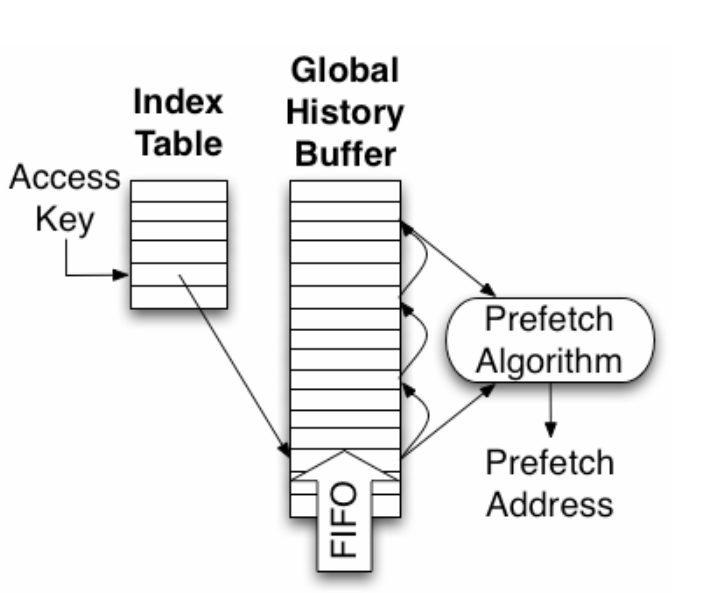
\includegraphics[scale=0.4]{images/GHB.png}}\par\medskip
 \caption{Global history buffer~\cite{Data Cache Prefetching Using a Global   History Buffer}}
 \label{fig:ghb}
 \end{figure}
 The GHB holds the $n$ most recent L2 cache miss addresses. Each GHB entry stores a global miss address and a link pointer. The link pointers are used to chain the GHB entries that form a time-ordered sequence of addresses having the same index table key. Depending on the key that is 
 used for indexing table, any history-based prefetch method can be realized. 

 \section{SPP}

SPP can predict multiple delta or stride values and complex strides across physical page boundaries~\cite{SPP}. It stores the memory access patterns in a compressed form called signatures. It also uses a confidence-based mechanism to throttle the aggressiveness of the prefertcher.
It uses a combination of the previous delta values for each page as a signature to index into a pattern table which gives the next delta and its confidence.
SPP uses a signature table to store the signatures and a pattern table for storing the delta values and their corresponding confidences~(Figure~\ref{fig:spp}). \begin{figure}[H]
{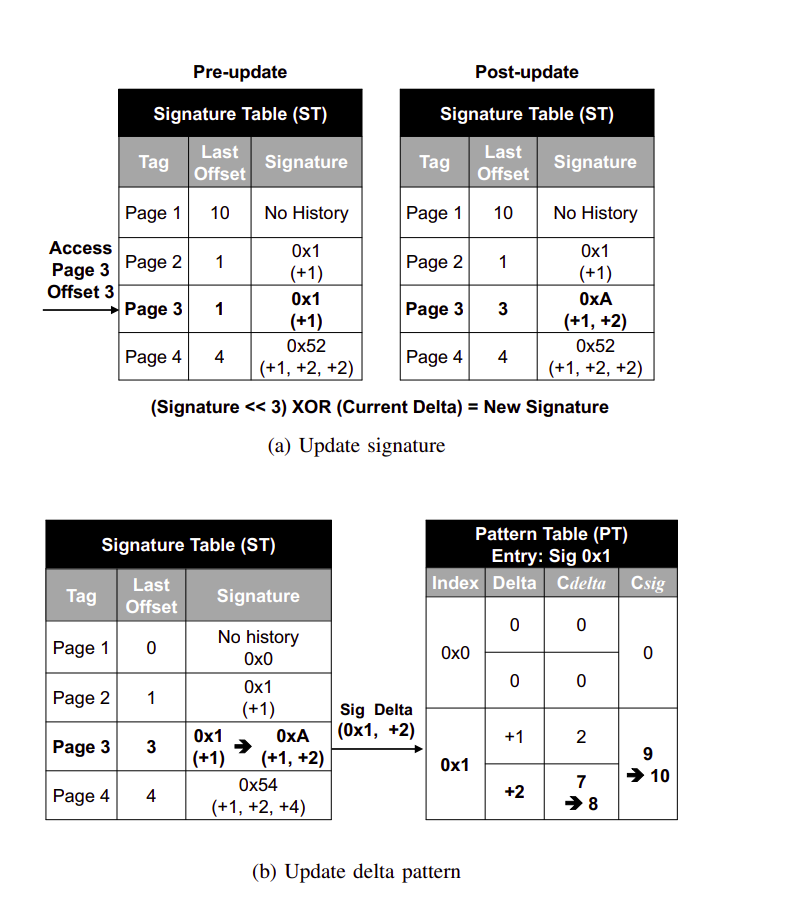
\includegraphics[scale=0.6]{images/SPP1.png}}
\caption{SPP operations~\cite{SPP}}
\label{fig:spp}
\end{figure}

Delta is used to generate the new signature, which is used to again access the pattern table to generate lookahead prefetches untill the path confidence falls below a threshold~(Figure~\ref{fig:spp2}). By using this mechanism SPP can learn complex access streams.
\begin{figure}[H]
{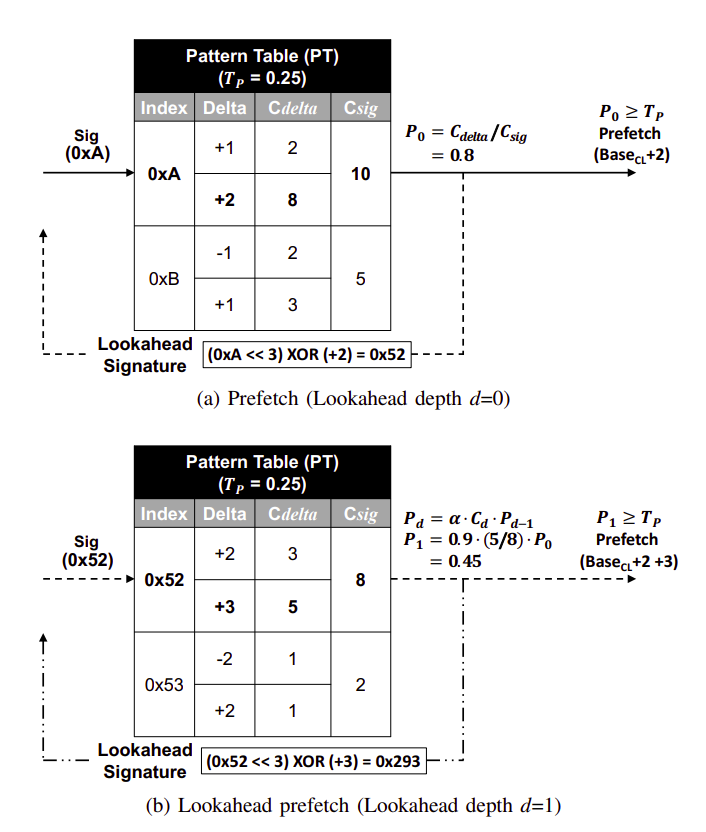
\includegraphics[scale=0.6]{images/SPP2.png}}
\caption{SPP delta and pattern table updates~\cite{SPP}}
\label{fig:spp2}
\end{figure}

\section{ Prefetch Filtering}

A very high degree of prefetching can result in cache pollution where useful cache blocks are replaced by unnecessarily early prefetches. On the other hand, a very low degree may not be able to take advantage of prefetching and may result in low coverage. There are types of workloads and phases of execution of the same workload which need prefetches with higher depth, while other workloads or phases may not require high depth. There are many techniques which reduce the cache pollution caused by aggressive prefetching. The general approach is to apply filtering mechanisms on the incoming prefetches or the outgoing prefetch requests. These mechanisms discard potentially less useful prefetches or prefetch them only to the bigger outer levels of the cache hierarchy where the negative impact of cache pollution may be low. One of the recent prefetch filters employs perceptrons to classify prefetches into useful and useless for filtering purpose~\cite{Perceptron filtering}. The proposal uses SPP as the underlying prefetcher, turns it more aggressive, and then uses multiple weight tables indexed using different features to implement a perceptron-based prefetch filter. Depending on the sum of the table outputs compared against a predecided threshold the filter decides whether to reject or go on with a prefetch.

Prior work on prefetch filtering has employed a dynamic feedback mechanism derived using prefetcher accuracy, prefetcher timeliness, and prefetcher-caused cache pollution~\cite{Feedback Directed Prefetching}. This feedback is used to adjust the aggressiveness of the prefetcher dynamically. This study also introduced a mechanism for estimating cache pollution and used this to decide the location in the LRU stack where a prefetched block should be inserted.  

%\section{Simulator and workloads}
%We have used a popular simulator \cite{Champsim}Champsim for simulations.  And the workloads used are \cite{SPEC2017}SPEC 2017. We have simulated our code for 1-core and 4-core configuration with 200M instructions. Our code of modified champsim simulator  can be found at \cite{git}.
